%============================================================
%  Capitolo 9 – Migliorare la Generalizzazione
%============================================================
\chapter{Migliorare la Generalizzazione}
\label{ch:generalization}

Addestrare una rete neurale significa minimizzare la funzione di perdita sul
training set. Ma l'obiettivo reale è ottenere buone prestazioni su dati
\emph{mai visti} durante l'addestramento. La differenza tra errore di training
ed errore di test prende il nome di \textbf{gap di generalizzazione}: ridurlo è
il problema centrale del Deep Learning applicato \citep{bishop2024}.

%------------------------------------------------------------
\section{Il Problema dell'Overfitting}
\label{sec:overfitting-recap}

I dati di addestramento contengono due tipi di informazione:

\begin{enumerate}
  \item \textbf{Regolarità reali}: la struttura autentica della mappatura
        input→output che il modello deve apprendere.
  \item \textbf{Errore di campionamento}: fluttuazioni accidentali dovute al
        particolare sottoinsieme di esempi scelto per il training.
\end{enumerate}

Il modello non può distinguere tra le due: \emph{fitta entrambe}. Se la rete ha
capacità elevata, riesce a modellare anche il rumore campionario molto bene,
producendo curve di addestramento quasi perfette ma generalizzazione scarsa.
Questo fenomeno è l'\textbf{overfitting}.

\paragraph{Tre approcci principali per prevenirlo.}
\begin{description}
  \item[Più dati] Raccogliere ulteriori esempi è quasi sempre la strategia più
        efficace: con dati abbondanti l'errore di campionamento si riduce e il
        modello è costretto ad apprendere le regolarità vere.
  \item[Capacità giusta] Usare un'architettura abbastanza grande da catturare le
        regolarità reali, ma non tanto da fittare il rumore.
  \item[Media di modelli] Combinare le predizioni di molti modelli diversi riduce
        la varianza senza aumentare il bias.
\end{description}

%------------------------------------------------------------
\section{Metodi per Limitare la Capacità}
\label{sec:limit-capacity}

La \textbf{capacità effettiva} di una rete può essere controllata lungo
quattro assi, spesso combinati tra loro:

\begin{description}
  \item[Architettura] Limitare il numero di layer nascosti e di unità per layer.
        È la forma più diretta di controllo ma richiede una ricerca manuale
        dell'architettura ottimale.
  \item[Early stopping] Interrompere l'addestramento prima che il modello
        inizi a fittare il rumore di campionamento (Sezione
        \ref{sec:early-stopping}).
  \item[Weight decay] Penalizzare i pesi grandi con un termine aggiuntivo
        alla loss (Sezione \ref{sec:weight-decay}).
  \item[Rumore] Aggiungere rumore ai pesi o alle attivazioni durante il
        training (Sezione \ref{sec:noise-regularizer}).
\end{description}

%------------------------------------------------------------
\section{Early Stopping}
\label{sec:early-stopping}

\subsection{Intuizione: Capacità come Funzione dei Pesi}
\label{subsec:early-stopping-intuition}

Quando i pesi sono molto piccoli, ogni unità nascosta opera nella sua
\textbf{regione lineare}: l'attivazione sigmoide o tanh si comporta
approssimativamente come una funzione lineare per piccoli argomenti. Una
rete con sole trasformazioni lineari ha capacità espressiva limitata,
equivalente a un singolo layer lineare.

Man mano che i pesi crescono, le unità nascono a utilizzare la propria
\textbf{regione non lineare}, aumentando la capacità della rete. L'early
stopping sfrutta questa dinamica: partendo da pesi piccoli e interrompendo
l'addestramento abbastanza presto si ottiene una rete con capacità
efficace \emph{limitata}, anche se l'architettura dichiarata sarebbe molto
capiente.

\begin{figure}[H]
  \centering
  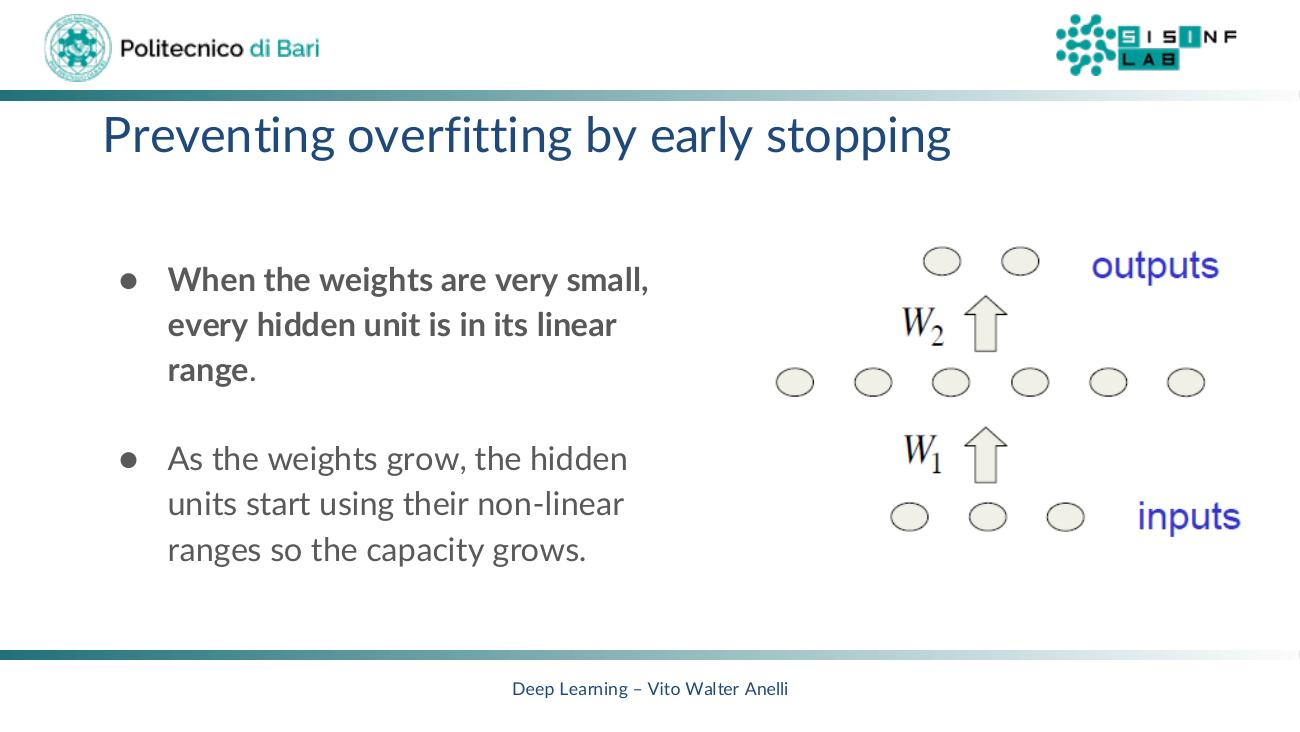
\includegraphics[width=0.72\linewidth]{figures/cf09_early_stopping_capacity.jpg}
  \caption{Early stopping e capacità. Con pesi piccoli ($W_1, W_2 \approx 0$)
           le unità nascoste sono nel regime lineare (bassa capacità). Al
           crescere dei pesi entrano nel regime non lineare e la capacità
           aumenta: fermarsi prima limita implicitamente la complessità del
           modello.}
  \label{fig:early_stopping}
\end{figure}

\subsection{Procedura Pratica}
\label{subsec:early-stopping-procedure}

\begin{enumerate}
  \item Tenere un \textbf{validation set} separato dal training set.
  \item Monitorare la validation loss a ogni epoch (o a intervalli regolari).
  \item Salvare i pesi ogni volta che la validation loss raggiunge un nuovo
        minimo (\emph{checkpoint}).
  \item Interrompere l'addestramento quando la validation loss non migliora
        per $k$ epoch consecutive (\emph{patience} $k$).
  \item Ripristinare i pesi del checkpoint migliore.
\end{enumerate}

\paragraph{Nota.} L'early stopping è concettualmente equivalente a una forma
di \emph{regolarizzazione implicita}: il numero di passi di aggiornamento svolge
lo stesso ruolo del coefficiente di penalizzazione in un problema di
ottimizzazione vincolata \citep{bishop2024}.

%------------------------------------------------------------
\section{Weight Decay (Regolarizzazione L2 e L1)}
\label{sec:weight-decay}

\subsection{Penalità L2}
\label{subsec:l2-penalty}

La \textbf{regolarizzazione L2} (o weight decay) aggiunge alla funzione di
costo un termine proporzionale alla somma dei quadrati dei pesi:

\begin{equation}
  \widetilde{\mathcal{L}}(\mathbf{w}) = \mathcal{L}(\mathbf{w})
    + \frac{\lambda}{2}\,\|\mathbf{w}\|^2
  = \mathcal{L}(\mathbf{w}) + \frac{\lambda}{2}\sum_i w_i^2.
  \label{eq:l2-loss}
\end{equation}

Il gradiente del termine di penalizzazione è $\lambda\,\mathbf{w}$, che si
sottrae ad ogni aggiornamento:

\begin{equation}
  w_i \leftarrow w_i - \eta\,\frac{\partial \mathcal{L}}{\partial w_i}
              - \eta\,\lambda\, w_i
  = w_i\,(1 - \eta\,\lambda) - \eta\,\frac{\partial\mathcal{L}}{\partial w_i}.
  \label{eq:l2-update}
\end{equation}

Il fattore $(1-\eta\lambda)$ riduce il peso ad ogni passo: i pesi rimangono
piccoli a meno che non contribuiscano a ridurre la loss, cioè a meno che
$\partial\mathcal{L}/\partial w_i$ sia grande. La penalità L2 corrisponde a
una \textbf{prior gaussiana} $p(w_i) \propto \exp(-\lambda w_i^2 / 2)$ nella
prospettiva bayesiana.

\subsection{Penalità L1}
\label{subsec:l1-penalty}

La \textbf{regolarizzazione L1} penalizza il valore assoluto dei pesi:

\begin{equation}
  \widetilde{\mathcal{L}}(\mathbf{w}) = \mathcal{L}(\mathbf{w})
    + \lambda\,\|\mathbf{w}\|_1
  = \mathcal{L}(\mathbf{w}) + \lambda\sum_i |w_i|.
  \label{eq:l1-loss}
\end{equation}

L'aggiornamento coinvolge il segno del peso:

\begin{equation}
  w_i \leftarrow w_i - \eta\,\frac{\partial\mathcal{L}}{\partial w_i}
              - \eta\,\lambda\,\operatorname{sign}(w_i).
  \label{eq:l1-update}
\end{equation}

La L1 tende a produrre soluzioni \textbf{sparse}: molti pesi vengono azzerati
esattamente. Equivale a una prior di Laplace $p(w_i) \propto
\exp(-\lambda|w_i|)$ e trova applicazione quando si desidera selezionare
automaticamente le feature rilevanti.

\begin{table}[H]
  \centering
  \caption{Confronto tra penalità L1 e L2.}
  \label{tab:l1-vs-l2}
  \small
  \begin{tabular}{lll}
    \toprule
    \textbf{Proprietà} & \textbf{L2 (Ridge)} & \textbf{L1 (Lasso)} \\
    \midrule
    Formula & $\lambda\sum w_i^2$ & $\lambda\sum |w_i|$ \\
    Effetto & Pesi piccoli ma non zero & Pesi sparsi (molti $= 0$) \\
    Prior bayesiana & Gaussiana & Laplace \\
    Derivabilità & Sì & No in $w_i=0$ \\
    Feature selection implicita & No & Sì \\
    Implementazione PyTorch & \texttt{weight\_decay} in optimizer & Penalità manuale \\
    \bottomrule
  \end{tabular}
\end{table}

%------------------------------------------------------------
\section{Rumore come Regolarizzatore}
\label{sec:noise-regularizer}

\subsection{Rumore Gaussiano sugli Input e L2 Implicita}
\label{subsec:gaussian-noise}

Aggiungere rumore gaussiano $\mathcal{N}(0, \sigma_i^2)$ all'input $x_i$ di
una rete semplice con unità di output lineare produce un effetto
regolarizzante equivalente alla penalità L2. La varianza del rumore viene
\emph{amplificata} dal quadrato del peso $w_i$ prima di contribuire all'uscita:

\begin{align}
  \tilde{x}_i &= x_i + \epsilon_i, \quad \epsilon_i \sim \mathcal{N}(0,\sigma_i^2),
  \label{eq:noisy-input} \\
  \tilde{y}_j &= y_j + \mathcal{N}(0, w_i^2 \sigma_i^2).
  \label{eq:noisy-output}
\end{align}

Minimizzare l'errore quadratico medio con input rumorosi equivale a minimizzare
l'errore quadratico medio originale più un termine $\sum_i w_i^2 \sigma_i^2$,
che è proporzionale alla penalità L2.

\begin{figure}[H]
  \centering
  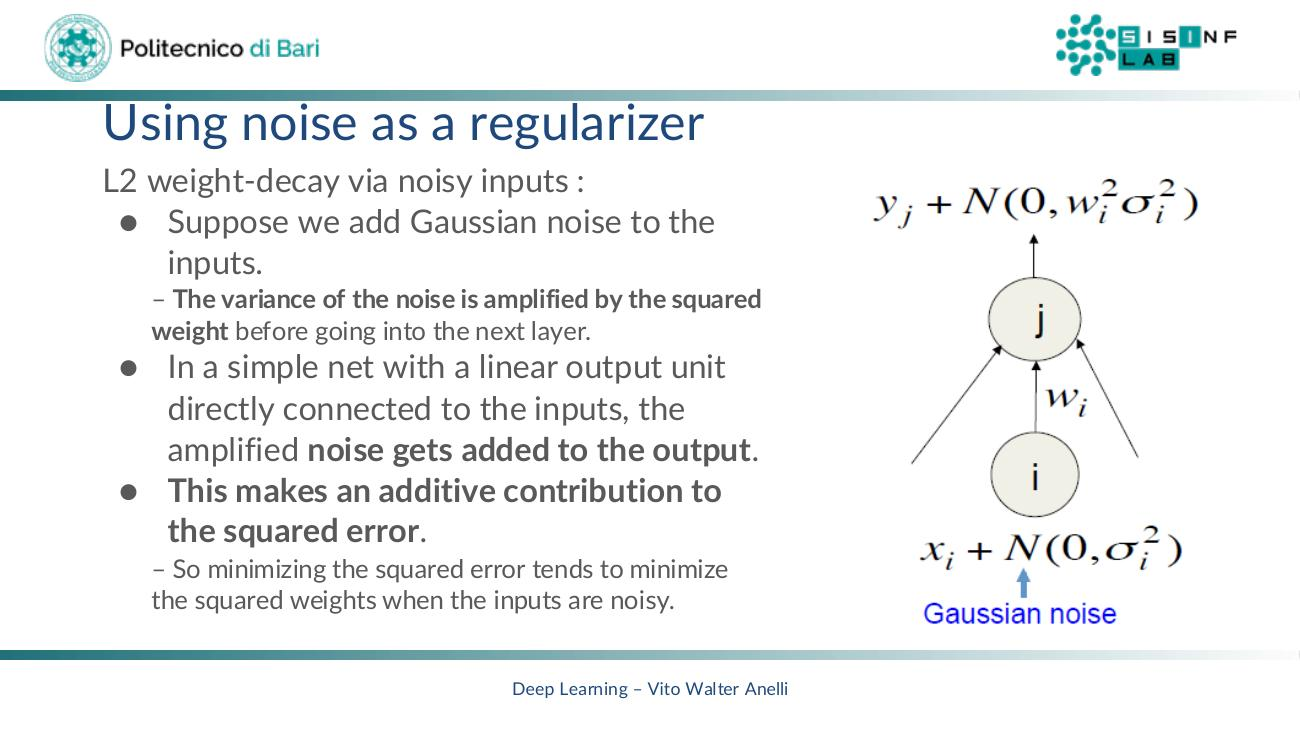
\includegraphics[width=0.62\linewidth]{figures/cf09_noise_regularizer.jpg}
  \caption{Rumore gaussiano come regolarizzatore L2. Il rumore sull'input
           $x_i \sim \mathcal{N}(0,\sigma_i^2)$ viene amplificato a
           $\mathcal{N}(0, w_i^2\sigma_i^2)$ nell'uscita $y_j$: minimizzare
           l'errore quadratico porta implicitamente a minimizzare $\sum_i w_i^2$.}
  \label{fig:noise_regularizer}
\end{figure}

\subsection{Forme di Rumore più Avanzate}
\label{subsec:advanced-noise}

Il rumore può essere applicato anche:
\begin{itemize}
  \item \textbf{Ai pesi} durante il forward pass: equivale ad una regolarizzazione
        sull'entropia della distribuzione dei pesi.
  \item \textbf{Alle attivazioni} dei layer nascosti: questa è la base del
        \textbf{Dropout} (Sezione \ref{sec:dropout}), dove il rumore ha la forma
        di una maschera binaria moltiplicativa.
\end{itemize}

%------------------------------------------------------------
\section{Combinare Modelli: Media degli Ensemble}
\label{sec:model-averaging}

\subsection{Bias-Variance Trade-off}
\label{subsec:bias-variance}

Per un problema di regressione, l'errore quadratico atteso si decompone in:

\begin{equation}
  \mathbb{E}\!\left[(y - \hat{y})^2\right]
  = \underbrace{\left(\mathbb{E}[\hat{y}] - y\right)^2}_{\text{Bias}^2}
  + \underbrace{\mathbb{E}\!\left[(\hat{y} - \mathbb{E}[\hat{y}])^2\right]}_{\text{Varianza}}
  + \sigma_\epsilon^2,
  \label{eq:bias-variance}
\end{equation}

dove $\sigma_\epsilon^2$ è la varianza del rumore irriducibile. La tabella
seguente riassume il trade-off:

\begin{table}[H]
  \centering
  \caption{Trade-off bias--varianza al variare della capacità del modello.}
  \label{tab:bias-variance}
  \small
  \begin{tabular}{lll}
    \toprule
    \textbf{Capacità} & \textbf{Bias} & \textbf{Varianza} \\
    \midrule
    Troppo bassa (underfitting) & Alto & Bassa \\
    Giusta & Basso & Bassa \\
    Troppo alta (overfitting) & Basso & Alta \\
    \bottomrule
  \end{tabular}
\end{table}

L'averaging di ensemble sfrutta il fatto che la \textbf{varianza di una media}
è inferiore alla varianza dei singoli modelli: combinando $M$ modelli
indipendenti con varianza $\sigma^2$ ciascuno si ottiene varianza $\sigma^2/M$.
Il bias invece non cambia. Si possono quindi usare modelli ad alta capacità
(basso bias, alta varianza) e ridurre la varianza via averaging
\citep{bishop2024}.

\subsection{Due Modi di Combinare i Modelli}
\label{subsec:mixture-product}

Dati $M$ modelli con distribuzione di output $P_m(y \mid \mathbf{x})$, esistono
due strategie di combinazione:

\paragraph{Mixture (media aritmetica).}
\begin{equation}
  P_{\text{mix}}(y \mid \mathbf{x}) = \frac{1}{M}\sum_{m=1}^{M} P_m(y \mid \mathbf{x}).
  \label{eq:mixture}
\end{equation}
La probabilità combinata è la media delle probabilità individuali. Corrisponde
a scegliere uniformemente uno dei modelli e campionare da esso.

\paragraph{Product (media geometrica).}
\begin{equation}
  P_{\text{prod}}(y \mid \mathbf{x}) \propto \prod_{m=1}^{M} P_m(y \mid \mathbf{x})
  = \exp\!\left(\frac{1}{M}\sum_{m=1}^{M} \log P_m(y \mid \mathbf{x})\right).
  \label{eq:product}
\end{equation}
La probabilità combinata è proporzionale al prodotto (o equivalentemente alla
media geometrica). È più \emph{conservativa}: assegna peso basso alle classi
che \emph{anche solo un} modello ritiene improbabili.

\begin{figure}[H]
  \centering
  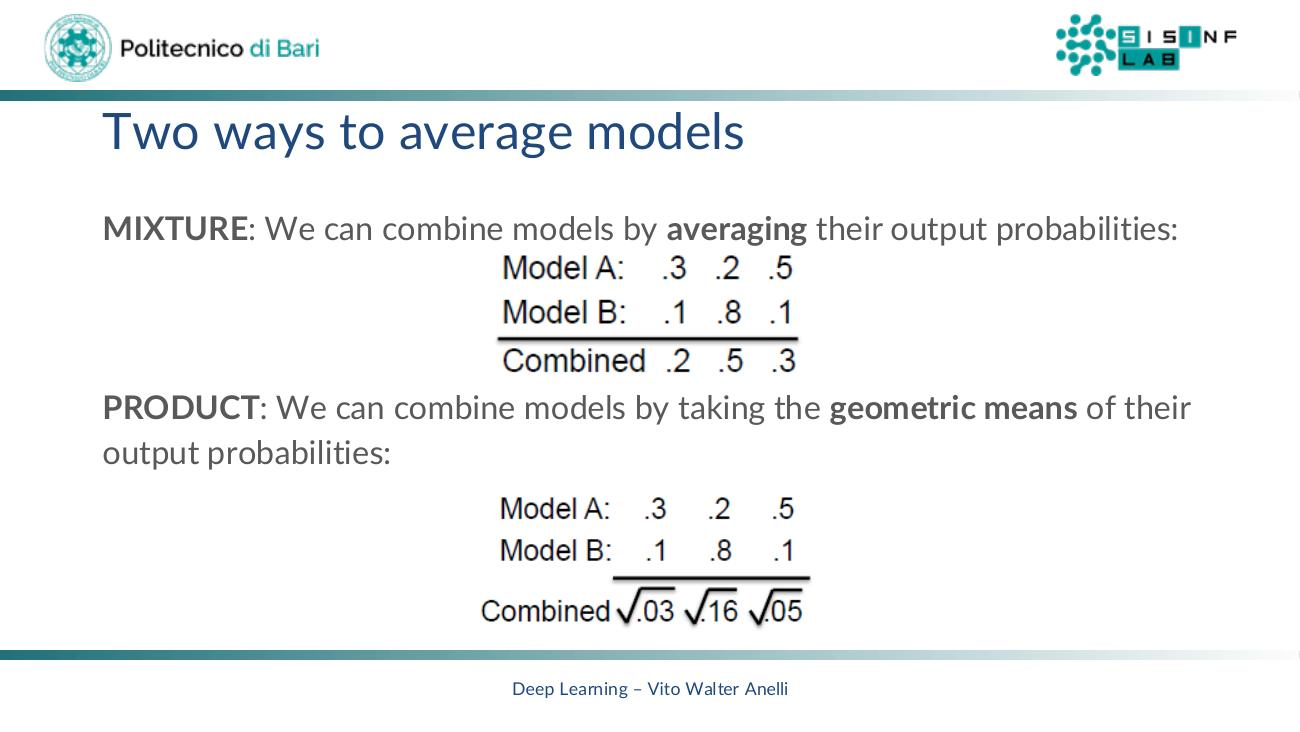
\includegraphics[width=0.70\linewidth]{figures/cf09_mixture_vs_product.jpg}
  \caption{Confronto numerico tra Mixture e Product su due modelli con tre
           classi. La mixture media aritmeticamente le probabilità; il product
           usa la media geometrica, producendo distribuzioni più concentrate
           sulle classi su cui i modelli concordano.}
  \label{fig:mixture_vs_product}
\end{figure}

\subsection{Come Rendere i Modelli Diversi}
\label{subsec:diverse-models}

Per massimizzare il beneficio dell'averaging, i modelli devono fare
\emph{errori diversi}. Le strategie principali sono:

\begin{description}
  \item[Bagging] Addestrare modelli diversi su sottoinsiemi estratti con
        rimpiazzo (\emph{bootstrap}). Le Random Forests applicano il bagging
        a alberi di decisione. Con reti neurali è molto costoso.
  \item[Boosting] Addestrare in sequenza modelli a bassa capacità, aumentando
        il peso degli esempi su cui i modelli precedenti hanno sbagliato. Focalizza
        le risorse computazionali sugli esempi difficili.
  \item[Diversità architetturale] Variare numero di layer, unità per layer,
        tipo di unità, tipo e forza della penalizzazione, algoritmo di
        ottimizzazione.
  \item[Diversità stocastica] Sfruttare la convergenza a minimi locali diversi
        in funzione dell'inizializzazione casuale (meno affidabile ma a costo zero).
\end{description}

%------------------------------------------------------------
\section{Dropout}
\label{sec:dropout}

\subsection{Definizione e Meccanismo}
\label{subsec:dropout-mechanism}

Il \textbf{Dropout} \citep{srivastava2014dropout} è una tecnica di
regolarizzazione che, a ogni forward pass durante il training, azzera
casualmente ciascuna unità nascosta con probabilità $p_{\text{drop}} = 1-p$
(dove $p$ è la \emph{keep probability}):

\begin{equation}
  \tilde{h}_i = m_i \cdot h_i, \quad
  m_i \sim \operatorname{Bernoulli}(p),
  \label{eq:dropout-mask}
\end{equation}

dove $\mathbf{m}$ è la \textbf{maschera} campionata indipendentemente per
ogni esempio e per ogni passo di training.

\begin{figure}[H]
  \centering
  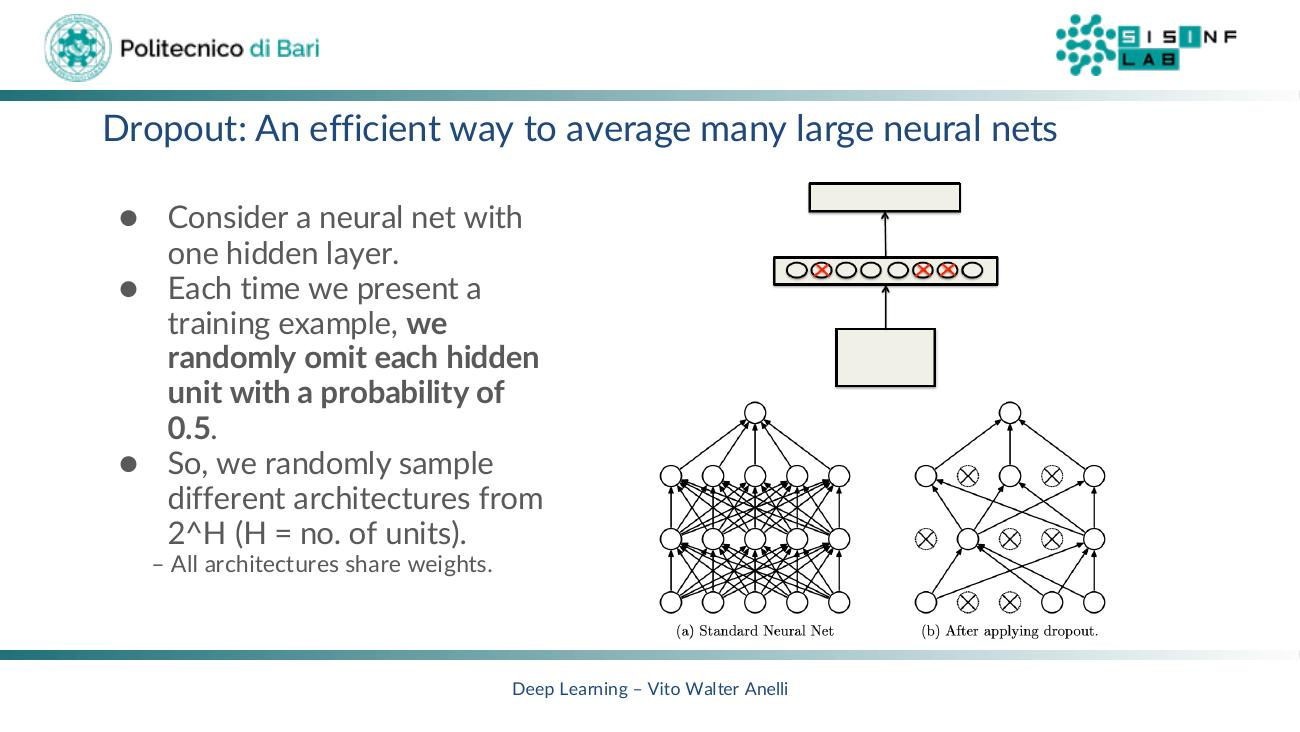
\includegraphics[width=0.82\linewidth]{figures/cf09_dropout_architecture.jpg}
  \caption{Dropout: (a) rete standard; (b) rete con dropout applicato -- le
           unità barrate (×) vengono annullate per quel forward pass. Con $H$
           unità nascoste si campiona tra $2^H$ sottoreti distinte, tutte con
           pesi condivisi.}
  \label{fig:dropout_arch}
\end{figure}

Con $H$ unità nascoste si esplorano fino a $2^H$ possibili sottoreti ad ogni
mini-batch. Tutte le sottoreti condividono gli stessi pesi, il che rappresenta
una regolarizzazione molto forte: ogni configurazione di pesi deve funzionare
bene per esponenzialmente molte architetture diverse.

\subsection{Dropout come Model Averaging}
\label{subsec:dropout-averaging}

Il Dropout può essere interpretato come una forma \emph{estrema} di bagging:
ogni sottorete viene addestrata su \emph{un solo} esempio (la configurazione di
maschera è unica per ogni forward pass). Rispetto al bagging classico i modelli
condividono però i pesi, il che li rende molto più fortemente regolarizzati di
quanto non farebbe la L2 o la L1 da soli.

\subsection{Inferenza a Tempo di Test: Weight Scaling}
\label{subsec:dropout-test}

Durante il test non si fa dropout: si usano \emph{tutte} le unità. Per
compensare il fatto che durante il training ogni unità era attiva solo con
probabilità $p$, i pesi in uscita vengono scalati:

\begin{equation}
  W_{\text{test}} = p \cdot W_{\text{train}}.
  \label{eq:weight-scaling}
\end{equation}

Questo garantisce che il valore atteso dell'attivazione a test time coincida
con quello a training time \citep{srivastava2014dropout}. In pratica, la
maggior parte dei framework (PyTorch, TensorFlow) implementa la variante
\textbf{inverted dropout}: durante il training i pesi \emph{attivi} vengono
divisi per $p$, così a test time non occorre alcun riscalamento:

\begin{equation}
  \tilde{h}_i = \frac{m_i \cdot h_i}{p}.
  \label{eq:inverted-dropout}
\end{equation}

\paragraph{Dropout multi-layer.}
Con più layer nascosti si applica dropout a ciascuno (tipicamente con $p = 0.5$
per i layer nascosti; $p = 0.8$--$0.9$ per il layer di input, che è più
sensibile alla perdita di features). Il modello medio (\emph{mean net}) con
tutti i pesi dimezzati non è esattamente la media geometrica di tutte le
sottoreti, ma è un'ottima approssimazione computazionalmente gratuita.

\paragraph{Dropout bayesiano (MC-Dropout).}
Eseguire il modello stocastico (con dropout attivo) $K$ volte sullo stesso
input durante il test fornisce una stima della \textbf{distribuzione di
incertezza} della predizione. Questa tecnica, nota come \emph{Monte Carlo
Dropout}, permette di quantificare l'incertezza predittiva senza richiedere
framework probabilistici complessi.

\subsection{Interpretazione della Co-Adattamento}
\label{subsec:coadaptation}

Un'unità nascosta che sa sempre quali altre unità sono presenti può
\emph{co-adattarsi}: specializzarsi in un compito che funziona solo in presenza
di un certo sottoinsieme di co-lavoratori. Tali co-adattazioni complesse sono
fragili su nuovi dati. Il Dropout rompe questo meccanismo: ogni unità deve
essere utile in combinazione con un insieme \emph{combinatorialmente diverso}
di co-lavoratori, il che la spinge a imparare feature autonomamente utili.

\begin{lstlisting}[language=Python, caption={Dropout in PyTorch.}, label={lst:dropout-pytorch}]
import torch.nn as nn

model = nn.Sequential(
    nn.Linear(d_in, d_h),
    nn.ReLU(),
    nn.Dropout(p=0.5),          # p = probabilita' di azzerare
    nn.Linear(d_h, d_h),
    nn.ReLU(),
    nn.Dropout(p=0.5),
    nn.Linear(d_h, d_out)
)

# Importante: attivare/disattivare il dropout correttamente
model.train()   # Dropout attivo
model.eval()    # Dropout disattivo (mean net)
\end{lstlisting}

%------------------------------------------------------------
\section{Riepilogo e Linee Guida Pratiche}
\label{sec:gen-summary}

\begin{table}[H]
  \centering
  \caption{Guida alla scelta della strategia di regolarizzazione.}
  \label{tab:regularization-guide}
  \small
  \begin{tabular}{lll}
    \toprule
    \textbf{Scenario} & \textbf{Strategia} & \textbf{Note} \\
    \midrule
    Dataset piccolo, modello semplice & L2 + Early Stopping & Baseline robusta \\
    Feature sparse / selezione & L1 (Lasso) & Produce pesi esattamente zero \\
    Reti profonde, dati medi & Dropout ($p=0.5$) & Standard per FC layers \\
    Reti convoluzionali & Batch Norm + Weight Decay & Dropout meno efficace nei conv \\
    Budget di compute limitato & Early Stopping & Costo zero aggiuntivo \\
    Incertezza predittiva & MC-Dropout & Stime probabilistiche \\
    Massima accuratezza disponibile & Ensemble + Dropout & Costoso ma efficace \\
    \bottomrule
  \end{tabular}
\end{table}

\paragraph{Regole operative.}
\begin{enumerate}
  \item Iniziare \textbf{sempre} con l'early stopping: non ha costo
        computazionale aggiuntivo e previene sprechi di addestramento.
  \item Aggiungere \textbf{weight decay} (L2) come regolarizzazione di base;
        usare AdamW che separa il weight decay dall'adattività del gradiente
        (cfr.\ Capitolo~\ref{ch:optimization}).
  \item Applicare \textbf{Dropout} nei layer fully-connected con $p = 0.5$;
        ridurre a $p = 0.2$--$0.3$ per layer convoluzionali o transformer,
        dove la ridondanza spaziale già regolarizza.
  \item Per la \textbf{stima dell'incertezza} usare MC-Dropout: fare $K = 30$
        --$100$ forward pass con dropout attivo e calcolare media e deviazione
        standard delle predizioni.
  \item Preferire \textbf{più dati} (o data augmentation) a regolarizzazioni
        aggressive: la regolarizzazione aiuta ma non sostituisce la ricchezza
        informativa del dataset.
  \item Ricordare di chiamare \texttt{model.eval()} prima dell'inferenza
        in PyTorch: altrimenti il Dropout rimane attivo e le predizioni
        risultano stocastiche e sub-ottimali.
\end{enumerate}

Come notato da \citet{bishop2024}, le tecniche di regolarizzazione non vanno
considerate alternative esclusive: la combinazione di early stopping, weight
decay e dropout è la norma nei moderni sistemi di deep learning ad alte
prestazioni.
